\notechapter{N-20210721}{A Gateway to Dualities: Space, Algebra, and the Dualizing Object}


\section{What could a space know about itself?}

Imagine a small world with three points $a,b,c$. We may forget their coordinates and even their names, yet still distinguish them by asking yes-or-no questions. Is a point in $\{a,b\}$? Answers may be combined by \emph{and}, \emph{or}, and \emph{not}, so all the questions form a Boolean algebra.

There is an attractive reversal of perspective here. Ordinarily we start with the points, construct the regions, and ask which regions contain a point. What if we start with the algebra of questions and try to recover the points themselves? A point ought to be a consistent way of answering \emph{every} question. It must say yes to the whole space, no to the empty set, and respect all the logical operations. The remarkable fact is that this idea reconstructs a space.

The finite experiment leads to Stone duality. Its more surprising descendants arise when questions are continuous functions, regular functions, or open sets, and eventually when truth itself can vary from one part of a space to another. The type of observation determines what sort of geometry can be recovered.

The exposition of the first duality follows Marcus Tressl's \href{https://personalpages.manchester.ac.uk/staff/marcus.tressl/papers/StoneDualityBooleanAlgebras.pdf}{\emph{Stone Duality for Boolean Algebras}}.


\section{Three points, eight regions, and three consistent answers}

For $X=\{a,b,c\}$ the algebra of all yes-or-no tests is
\[
 B=\mathcal P(X)
 =\{\varnothing,\{a\},\{b\},\{c\},
       \{a,b\},\{a,c\},\{b,c\},X\}.
\]
A point $x\in X$ defines an evaluation
\[
 e_x:B\longrightarrow\mathbf2=\{0,1\},
 \qquad e_x(U)=
 \begin{cases}1,&x\in U,\\0,&x\notin U.\end{cases}
\]
For instance $e_a(\{a,b\})=1$ whereas $e_c(\{a,b\})=0$. These three evaluations are precisely the Boolean homomorphisms $B\to\mathbf2$: each must select exactly one of the three mutually exclusive singleton atoms, and then all eight answers are forced.

\begin{figure}[H]
\centering
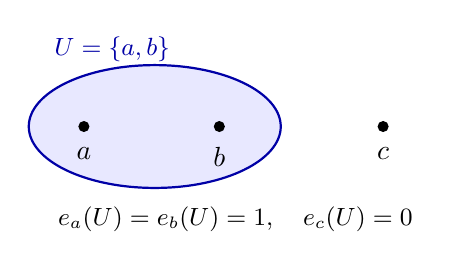
\begin{tikzpicture}[scale=1.0]
 \fill[blue!9] (-.55,0) ellipse (1.60 and .78);
 \draw[blue!65!black,thick] (-.55,0) ellipse (1.60 and .78);
 \fill (-1.45,0) circle (2pt) node[below=4pt] {$a$};
 \fill (.27,0) circle (2pt) node[below=4pt] {$b$};
 \fill (2.35,0) circle (2pt) node[below=4pt] {$c$};
 \node[blue!65!black,anchor=west,font=\small] at (-1.95,.98)
       {$U=\{a,b\}$};
 \node[font=\small,anchor=west] at (-1.9,-1.18)
       {$e_a(U)=e_b(U)=1,\quad e_c(U)=0$};
\end{tikzpicture}
\caption{A subset is a question; a point is an evaluation of that question. Boolean combinations of the eight subsets are compatible with exactly three evaluations.}
\end{figure}

This small calculation contains the ambition of duality: reconstruct points as mathematical objects \emph{defined by their observations}. It also suggests when reconstruction could fail: if the allowed questions cannot distinguish two points, the algebra cannot distinguish them either.


\section{A map reverses the direction of questions}

Let $f:X\to Y$ be a function. A test $V\subseteq Y$ can be performed on a point $x\in X$ by testing whether $f(x)\in V$. Thus a test on $Y$ becomes a test on $X$:
\[
 f^{-1}:\mathcal P(Y)\longrightarrow\mathcal P(X),
 \qquad V\longmapsto f^{-1}(V).
\]
For example, take $X=\{a,b,c\}$, $Y=\{u,v\}$ and
\[
 f(a)=f(b)=u,\qquad f(c)=v.
\]
The question about output $u$ pulls back to the question about inputs $a,b$:
\[
 f^{-1}(\{u\})=\{a,b\}.
\]
The reversed arrow is forced by the direction in which \emph{questions} travel.

More generally, for a target object $\Omega$, composition defines
\[
 \operatorname{Hom}(Y,\Omega)
 \xrightarrow{\ \varphi\mapsto\varphi\circ f\ }
 \operatorname{Hom}(X,\Omega).
\]
This is \emph{contravariance}: $(g\circ f)^*=f^*\circ g^*$.
It is a simple identity, but the right shape for a geometry-to-algebra correspondence.

For Stone duality, $\Omega=\mathbf2$ wears two compatible costumes. As a \emph{discrete topological space}, maps $X\to\mathbf2$ describe clopen regions; as a \emph{Boolean algebra}, homomorphisms $B\to\mathbf2$ describe consistent truth assignments. These Hom sets belong to different categories. Stone's theorem states that their constructions recover one another.

Reversing arrows by itself never proves a duality: reconstruction requires sufficiently many observations, an appropriate category of spaces, and the correct algebraic operations on those observations.

\section{Stone duality as the first complete example}

The first row is the best place to begin because it is the most logical and the most concrete:
\[
  \text{Stone spaces}\quad \longleftrightarrow\quad \text{Boolean algebras},
  \qquad
  \Omega=\mathbf 2=\{0,1\}.
\]
Here \(\mathbf 2\) is the space of truth values.  A map into \(\mathbf 2\) is a yes-or-no observation.

\subsection{Boolean algebras as propositional logic}

A Boolean algebra is an algebraic model of classical propositional logic.

\begin{definition}[Boolean algebra]
A Boolean algebra is a structure
\[
  B=(B,\vee,\wedge,{}',0,1)
\]
where \(\vee\) and \(\wedge\) are join and meet, \(0\) and \(1\) are bottom and top, and each element \(a\in B\) has a complement \(a'\).  It satisfies the usual associativity, commutativity, absorption, distributivity, and complementation laws.
\end{definition}

The example to keep in mind is the power set \(\mathcal P(X)\).  Then
\[
  A\vee B=A\cup B,
  \qquad
  A\wedge B=A\cap B,
  \qquad
  A'=X\setminus A.
\]
So Boolean algebra is the algebra of regions that can be combined by union, intersection, and complement.

\subsection{Stone spaces as spaces with Boolean topology}

A Stone space is a topological space whose topology is controlled by clopen sets.

\begin{definition}[Stone space]
A Stone space is a compact Hausdorff totally disconnected space.  Equivalently, it is a compact Hausdorff space with a basis of clopen subsets.
\end{definition}

A subset is clopen if it is both closed and open.  In ordinary connected spaces, clopen sets are rare.  In a Stone space, clopen sets are abundant enough to form the logical basis of the space.

For any Stone space \(X\), the clopen subsets form a Boolean algebra:
\[
  \operatorname{Clop}(X).
\]
The Boolean operations are exactly the set operations:
\[
  U\vee V=U\cup V,
  \qquad
  U\wedge V=U\cap V,
  \qquad
  U'=X\setminus U.
\]
This gives the direction
\[
  X\longmapsto \operatorname{Clop}(X).
\]

\subsection{Why \(\mathbf 2\) is the dualizing object}

The set \(\mathbf 2=\{0,1\}\) is given the discrete topology.  A continuous map
\[
  \chi:X\to \mathbf 2
\]
is the characteristic function of a clopen subset of \(X\).  Indeed,
\[
  \chi^{-1}(\{1\})
\]
is clopen because \(\{1\}\subset \mathbf 2\) is clopen.

Thus
\[
  \operatorname{Hom}_{\mathbf{Top}}(X,\mathbf 2)\cong \operatorname{Clop}(X).
\]
This is the first half of the row: the algebra of logic on a Stone space is the algebra of truth-valued continuous observations.

\subsection{Ultrafilters as points}

Now start from a Boolean algebra \(B\).  A point of the Stone space of \(B\) is not given in advance.  It must be reconstructed from the algebra.

\begin{definition}[Filter and ultrafilter]
A filter \(F\subseteq B\) is a subset such that \(1\in F\), \(0\notin F\), it is closed under finite meets, and it is upward closed.  An ultrafilter is a maximal proper filter.
\end{definition}

An ultrafilter is a complete truth assignment.  For every proposition \(a\in B\), exactly one of \(a\) and \(a'\) belongs to the ultrafilter.  So an ultrafilter decides every proposition in a way compatible with Boolean logic.

Let
\[
  S(B)=\{\mathfrak u : \mathfrak u\text{ is an ultrafilter on }B\}.
\]
For each \(a\in B\), define
\[
  U_a=\{\mathfrak u\in S(B):a\in\mathfrak u\}.
\]
The sets \(U_a\) form a basis of clopen subsets.  This turns \(S(B)\) into a Stone space.

The map
\[
  a\longmapsto U_a
\]
preserves Boolean operations:
\[
  U_{a\wedge b}=U_a\cap U_b,
  \qquad
  U_{a\vee b}=U_a\cup U_b,
  \qquad
  U_{a'}=S(B)\setminus U_a.
\]

\begin{theorem}[Stone representation theorem]
For every Boolean algebra \(B\), the map
\[
  B\longrightarrow \operatorname{Clop}(S(B)),
  \qquad
  a\longmapsto U_a
\]
is an isomorphism of Boolean algebras.
\end{theorem}

This is the missing geometric half of Boolean algebra.  A Boolean algebra is not only a symbolic calculus of propositions.  It is the algebra of clopen regions of a canonically reconstructed space.


\subsection{Why the reconstruction actually works}

The displayed Boolean operations are straightforward. The stronger assertion is that $a\mapsto U_a$ loses no information and produces \emph{all} clopen sets. Here is the mechanism.

If $a\ne b$, either $a\wedge b'\ne0$ or $b\wedge a'\ne0$. A nonzero Boolean element belongs to some ultrafilter; this is the ultrafilter extension principle, a form of the Boolean prime ideal theorem. Consequently, some ultrafilter contains exactly one of $a,b$. Their clopen regions $U_a,U_b$ differ. The map is injective.

For compactness, suppose the basic clopen sets $U_{a_i}$ cover $S(B)$ but no finite subfamily covers it. Then every finite meet of complements
\[
 a_{i_1}'\wedge\cdots\wedge a_{i_r}'\ne0.
\]
The complements have the finite-intersection property, so an ultrafilter contains all of them. It belongs to none of the $U_{a_i}$, contradicting the cover. Every basic cover thus has a finite subcover. The sets $U_a$ are clopen because $S(B)\setminus U_a=U_{a'}$, and distinct ultrafilters are separated by complementary clopens. Hence $S(B)$ is compact, Hausdorff, and zero-dimensional.

Finally, any clopen $C\subseteq S(B)$ is compact. The basic sets $U_a$ contained in $C$ cover it, and finitely many suffice:
\[
 C=U_{a_1}\cup\cdots\cup U_{a_r}
   =U_{a_1\vee\cdots\vee a_r}.
\]
This proves surjectivity. The ultrafilter extension principle is a genuine set-theoretic input for general Boolean algebras; the finite three-point example needed no such principle.

\subsection{An infinite example you can draw: the Cantor space}

Let $X=\{0,1\}^{\mathbb N}$ be the space of infinite binary sequences. To test a point, ask about only finitely many digits. For a finite word $w$, its \emph{cylinder}
\[
 [w]=\{x\in X:x_1\cdots x_{|w|}=w\}
\]
is clopen. Cylinders form a basis; every clopen subset is a \emph{finite} union of them, by compactness.

\begin{figure}[H]
\centering
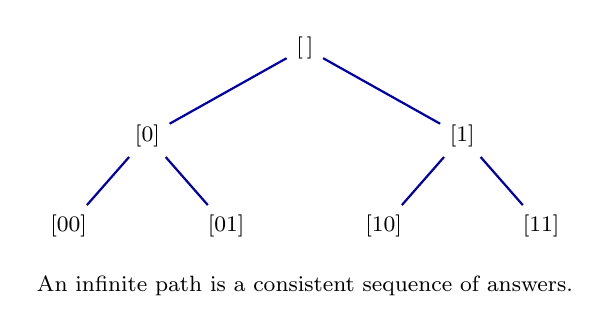
\begin{tikzpicture}[every node/.style={font=\footnotesize}]
 \node (r) at (0,1.72) {$[\,]$};
 \node (a) at (-2.0,.60) {$[0]$};
 \node (b) at (2.0,.60) {$[1]$};
 \node (aa) at (-3.0,-.54) {$[00]$};
 \node (ab) at (-1.0,-.54) {$[01]$};
 \node (ba) at (1.0,-.54) {$[10]$};
 \node (bb) at (3.0,-.54) {$[11]$};
 \draw[thick,blue!65!black] (r)--(a) (r)--(b);
 \draw[thick,blue!65!black] (a)--(aa) (a)--(ab)
                             (b)--(ba) (b)--(bb);
 \node[anchor=north,font=\footnotesize] at (0,-1.05)
  {An infinite path is a consistent sequence of answers.};
\end{tikzpicture}
\caption{Binary cylinder questions form a nested family. Their consistent infinite answers are precisely the points of the Cantor space.}
\end{figure}

A sequence $x=(x_1,x_2,\ldots)$ chooses, at every level, the unique cylinder recording its first digits. Conversely, any compatible chain $[x_1]\supseteq[x_1x_2]\supseteq\cdots$ singles out one infinite sequence. Coherent answers reconstruct a point even when there are infinitely many questions. The topology arises because two sequences are close when many early answers agree.


\section{Recovering maps as well as points}

A duality must reconstruct \emph{arrows}, not only objects. In the finite example, a function $f:X\to Y$ determines a Boolean homomorphism
\[
 f^{-1}:\mathcal P(Y)\to\mathcal P(X).
\]
Conversely, suppose $h:\mathcal P(Y)\to\mathcal P(X)$ is a Boolean homomorphism between the power-set algebras of finite sets. The singleton subsets $\{y\}$ of $Y$ are pairwise disjoint and their union is $Y$. Therefore the sets $h(\{y\})$ partition $X$ (some may be empty). Each $x\in X$ belongs to exactly one of these sets. Define $f(x)$ to be that unique $y$. The homomorphism is necessarily $h=f^{-1}$.

In the general case, a Boolean homomorphism $h:B\to C$ sends each ultrafilter of $C$ to its inverse-image ultrafilter in $B$. Hence it induces a continuous map
\[
 S(C)\longrightarrow S(B),\qquad
 \mathfrak u\longmapsto h^{-1}(\mathfrak u).
\]
The direction reverses again. Stone duality is the contravariant equivalence
\[
 \boxed{\mathbf{Stone}\simeq\mathbf{Bool}^{\mathrm{op}}.}
\]
Points become consistent truth assignments, predicates become clopen regions, and maps become substitution of predicates. This is a precise sense in which Boolean logic has a topology.


\section{What happens when yes-or-no questions are too poor?}

Take the connected interval $X=[0,1]$. Its only clopen subsets are $\varnothing$ and $X$. If we observe a point only through continuous maps to the \emph{discrete} space $\mathbf2$, then every observation is constant. We cannot tell $0$ from $1/2$.

A simple repair is to use \emph{complex-valued continuous functions}. The coordinate function $t\mapsto t$ distinguishes every pair of points on the interval. For a compact Hausdorff space $X$, let $C(X)$ denote the continuous functions $X\to\mathbb C$, with pointwise operations, complex conjugation, and
\[
 \|h\|_\infty=\sup_{x\in X}|h(x)|.
\]
This is a commutative unital $C^*$-algebra: the norm and involution remember precisely the analytic structure we want.

Every point $x$ determines an evaluation character
\[
 \operatorname{ev}_x:C(X)\to\mathbb C,\qquad h\mapsto h(x).
\]
A character here is a nonzero unital multiplicative complex-linear functional, and in the $C^*$ setting it respects the $*$-structure. Gelfand's theorem says that for compact Hausdorff $X$, every character of $C(X)$ is evaluation at a unique point. In this setting functions separate points and remember the topology.

\begin{theorem}[Commutative Gelfand duality]
The category of compact Hausdorff spaces is contravariantly equivalent to the category of commutative unital complex $C^*$-algebras and unital $*$-homomorphisms. In particular, for such an algebra $A$,
\[
 \boxed{A\cong C(\operatorname{Spec}A),}
\]
where $\operatorname{Spec}A$ is its compact Hausdorff space of characters.
\end{theorem}

The finite case can be seen without functional analysis. If $X=\{p,q\}$, then $C(X)\cong\mathbb C^2$. A unital multiplicative functional to $\mathbb C$ must evaluate one of the two factors, because the idempotents $(1,0)$ and $(0,1)$ have images in $\{0,1\}$ and sum to $1$. The characters are exactly $\operatorname{ev}_p,\operatorname{ev}_q$.

A continuous map $f:X\to Y$ again turns observations on $Y$ into observations on $X$:
\[
 f^*:C(Y)\to C(X),\qquad h\longmapsto h\circ f.
\]
For $f(t)=t^2$ on $[0,1]$, the observable $h(t)=t$ is pulled back to $h\circ f(t)=t^2$. The same contravariant pattern has acquired analytic information. The difference from Stone duality is substantial: a complex-valued observable carries far more than a binary truth value.


\section{A polynomial remembers points that ordinary values miss}

Continuous functions suggest another sort of observation: \emph{regular functions} in algebraic geometry. An affine scheme is of the form $X=\operatorname{Spec}R$ for a commutative ring $R$. Its points are prime ideals of $R$, and the basic open sets are
\[
 D(f)=\{\mathfrak p\in\operatorname{Spec}R:f\notin\mathfrak p\}.
\]
Ring homomorphisms run opposite to geometric maps:
\[
 \varphi:R\to S
 \quad\rightsquigarrow\quad
 \operatorname{Spec}S\to\operatorname{Spec}R,
 \qquad\mathfrak q\mapsto\varphi^{-1}(\mathfrak q).
\]

Why prime ideals rather than just numerical solutions? Consider $R=k[t]$, with $k$ algebraically closed. The maximal ideals $(t-a)$ are the familiar points $a\in k$, but the zero ideal $(0)$ is also prime. This \emph{generic point} lies in every nonempty basic open set. It encodes the whole irreducible affine line rather than a particular value of $t$.

The ring of functions is recovered using the structure sheaf:
\[
 \Gamma(\operatorname{Spec}R,\mathcal O)=R,
 \qquad
 \Gamma(D(f),\mathcal O)=R_f.
\]
For example, over $k[t]$ the open region where $t\ne0$ admits regular functions such as $t^{-1}$, even though $t^{-1}$ is not regular on the whole line.

The \emph{affine line scheme} $\mathbb A^1_{\mathbb Z}=\operatorname{Spec}\mathbb Z[t]$ gives a particularly attractive version of the observation principle:
\[
 \boxed{\operatorname{Hom}_{\mathbf{Sch}}
       (X,\mathbb A^1_{\mathbb Z})
       \cong\Gamma(X,\mathcal O_X).}
\]
For an affine $X=\operatorname{Spec}R$, this is $R$ itself: a scheme map to the affine line is determined by the image of its coordinate $t$, hence by a global function. The computation uses the scheme structure, not merely the underlying point set.

Indeed two affine schemes can have the same underlying topological space and different algebras. The ring of dual numbers
\[
 R=k[\varepsilon]/(\varepsilon^2)
\]
has one prime ideal $(\varepsilon)$, so $\operatorname{Spec}R$ has just one topological point. Its global sections still contain a nonzero element $\varepsilon$ with $\varepsilon^2=0$. The scheme $\operatorname{Spec}k$ has the same one-point topology but lacks that infinitesimal direction. Forgetting the sheaf would lose exactly the information that algebraic geometry needs.

The precise duality is between \emph{affine schemes} and commutative rings, with arrows reversed. The equivalence does not assert that arbitrary schemes are determined by a single ring of global functions. See the Stacks Project, \href{https://stacks.math.columbia.edu/tag/01HR}{\emph{Affine Schemes}}, for the local-section calculation.


\section{Why an open set is a different kind of truth}

A clopen predicate has a continuous characteristic function into discrete $\mathbf2$. To represent an \emph{arbitrary open} predicate, the target must change its topology.

Let $\mathbb S=\{0,1\}$ have opens
\[
 \mathcal O(\mathbb S)=\{\varnothing,\{1\},\mathbb S\}.
\]
This is the Sierpi\'nski space. For any topological space $X$, the function $\chi_U:X\to\mathbb S$ that equals $1$ on $U$ and $0$ outside is continuous exactly when $U$ is open:
\[
 \boxed{\operatorname{Hom}_{\mathbf{Top}}(X,\mathbb S)
            \cong\mathcal O(X).}
\]
One of the two truth values is observable as an open condition; the other need not be. For $U=(0,\infty)\subset\mathbb R$, the characteristic function is continuous into $\mathbb S$, but not into discrete $\mathbf2$. This single example explains the asymmetric topology of $\mathbb S$.

The algebra of all opens $\mathcal O(X)$ is a \emph{frame}: arbitrary unions exist, finite intersections distribute over arbitrary unions, and
\[
 U\cap\bigcup_i V_i=\bigcup_i(U\cap V_i).
\]
A continuous map $f:X\to Y$ gives a frame homomorphism
\[
 f^{-1}:\mathcal O(Y)\longrightarrow\mathcal O(X).
\]
A locale is a space described directly by such a frame. Thus locales and frames are opposites by their defining conventions. Recovering an actual point-set space from the frame of opens requires a further hypothesis, such as sobriety; point-free locales need not be spatial.

This is a close cousin of the Stone construction, with an important change of expressive power. Clopens encode Boolean logic, where complement always stays open. General opens encode a Heyting algebra, where the logical negation of $U$ is the interior of its complement, $\operatorname{int}(X\setminus U)$.


\section{A truth value can vary across a space}

A sheaf makes the local character of topology tangible. For each open region $U\subseteq X$, a sheaf $\mathcal F$ assigns a set $\mathcal F(U)$ of data available over $U$, together with restriction maps when $V\subseteq U$. Compatible local data may be glued. The category $\mathbf{Sh}(X)$ of sheaves is an example of a \emph{topos}.

The truth-value object of a topos is called its \emph{subobject classifier} $\Omega$. In $\mathbf{Set}$ it is simply $\{0,1\}$. In the sheaf topos $\mathbf{Sh}(X)$, it has a beautiful local description:
\[
 \boxed{\Omega(U)=\{V:V\subseteq U,\ V\text{ open}\}.}
\]
Restriction from $U$ to $W$ sends $V$ to $V\cap W$. An assertion can be true over one open patch without being true everywhere, and its truth value is the patch on which it holds.

Here is a concrete logical phenomenon. Let $X=\mathbb R$ and take the proposition that the real coordinate is positive. Its truth value is the open set
\[
 P=(0,\infty).
\]
The internal negation corresponds to the largest open set disjoint from $P$:
\[
 \neg P=\operatorname{int}(\mathbb R\setminus P)=(-\infty,0).
\]
Therefore
\[
 P\vee\neg P=\mathbb R\setminus\{0\}\ne\mathbb R.
\]
At the boundary point $0$, neither side is locally forced. This is the first glimpse of \emph{intuitionistic} internal logic: truth can be local, and Boolean complementation is too strong for general open information.

The deeper language of topoi, including classifying topoi and higher topoi, develops these themes in categorical and homotopical directions. The term \emph{logos} is used for particular logical presentations in higher category theory, but there is no general identity obtained by putting $\mathbf{Set}$ into both sides of $\operatorname{Hom}(-,\Omega)$ and declaring every topos to be its dual. What survives from the elementary examples is the structural question: which tests describe a space, and what reconstruction theorem, if any, makes the description complete?

A standard reference for the connection between sheaves and internal logic is Saunders Mac Lane and Ieke Moerdijk, \emph{Sheaves in Geometry and Logic}.


\section{A duality remembers both the object and its maps}

The category-theoretic content is an equivalence $\mathcal C\simeq\mathcal D^{\mathrm{op}}$. Two contravariant constructions must reconstruct objects up to natural isomorphism and maps compatibly with composition. The simplest warning is our connected interval: maps $[0,1]\to\mathbf2$ with $\mathbf2$ discrete cannot distinguish its points, so this particular family of tests does not reconstruct it. Replacing the tests by continuous complex-valued functions restores far more information.

The main correspondences have different exact domains:
\[
\begin{array}{c|c}
 \text{space-like side} & \text{algebraic side}\\ \hline
 \text{Stone spaces} & \text{Boolean algebras}\\
 \text{compact Hausdorff spaces} & \text{unital commutative }C^*\text{-algebras}\\
 \text{affine schemes} & \text{commutative rings}\\
 \text{locales} & \text{frames}
\end{array}
\]
Each row reverses arrows, but the reconstruction theorems are different. The discrete two-point object measures clopen predicates; $\mathbb C$ measures continuous functions; the affine line represents regular functions; the Sierpi\'nski space represents open predicates. Inside a topos, the subobject classifier $\Omega$ classifies subobjects, and its truth values may themselves vary over a base space. These are related forms of mathematical observation, with distinct hypotheses.

The sequence of examples can now be read from the perspective of the three-point world. We began by recovering a point from all its yes-or-no answers. Then we allowed continuously varying answers to distinguish points of connected spaces. In algebraic geometry the answers were regular functions and even infinitesimal data; in locale theory they were open conditions; in sheaf theory an answer itself became local.

The reversal of arrows is easy: an observation of $Y$ can always be pulled back along a map $X\to Y$. The beautiful part is \emph{recoverability}. When the observations encode exactly the right structure, points and maps reappear from what they do to all possible questions.
